\begin{savequote}[75mm]
Searle may only be behaving \textit{as if} he were thinking deeply about these matters. But, even though I disagree with him, his simulation is pretty good, so I'm willing to credit him with real thought.\qauthor{Nils Nilsson}
\end{savequote}

\chapter{Luna Rating Prediction}

\section{Introduction}
\subsection{The Luna Rating Prediction Problem}
In the previous chapter, I discussed the machine learning problems implicit in the Interview and Response phases of the Luna Game. This chapter addresses the remaining problem implied by the Guess phase. Consider the typical behavior of a human player during this phase. The player observes her opponent's responses. If she has asked the same questions to previous opponents, she may compare these new responses to old responses, and conjecture that opponents who respond similarly have similar Smarts Ratings. In addition, she may compare these new responses directly with the ideal responses that she had in mind, reasoning that opponents who provide ideal responses are likely to have high Smarts Ratings. After taking into account all the information at her disposal --- previously observed responses and previously conceived ideal answers --- she hazards a guess.

The task implicit in the Guess phase is best clarified in terms independent from the Luna Game. The goal is to learn a mapping from ordered sets of natural language samples to a bounded subset of the real numbers that minimizes ($L_1$) error on test data. Given the inspiration of this problem, I call it the Luna Rating Prediction (LRP) problem. In this chapter, I present a collection of simple experiments to establish a baseline for the problem. I conclude with a discussion of avenues for future work and an argument for LRP's general applicability beyond the scope of Luna.

LRP avoids some of the difficulties of natural language understanding, but also introduces a host of new challenges. For example, it is possible in principal to achieve very good results on LRP without a complete understanding of the natural language responses being analyzed. On the other hand, a complete understanding of the responses is not sufficient to solve LRP, since ratings must still be predicted. Machines may excel at mapping representations of responses to ratings, while humans may excel at representing the responses. A method for LRP must excel at both tasks.

\subsection{Related Work}
LRP may be viewed as a relaxed version of a problem that has been previously considered: Automatic Short Answer Grading (ASAG) \cite{burrows2015eras, pulman2005automatic, sukkarieh2009c, ziai2012short}. Motivated by standardized testing, ASAG attempts to grade student responses to a fixed set of questions. While LRP is concerned only with the cumulative rating of all responses for a particular respondent, ASAG requires scores for each question. If player ratings are assumed to be completely determined based on their responses to the given set of questions, then LRP reduces to ASAG. In this scenario, a solution to ASAG would imply a solution to LRP, but LRP may be solved without solving ASAG. For example, if one question is much more predictive of a respondent's overall rating than other questions, LRP would be able to leverage this correspondence, while ASAG would be forced to grade all questions, each contributing equally to overall error. 

Previous work on ASAG provides a baseline for work on LRP. A recent review by Burrows et al. summarizes advances in ASAG, drawing upon over 80 papers with 35 distinct systems \cite{burrows2015eras}. These systems differ in their natural language processing techniques, model building, grading models, and effectiveness. Each of these systems could be potentially adapted for LRP, offering several possible avenues for future research. Here I focus on the state-of-the-art system developed by Education Testing Services \cite{heilman2013ets}. This system serves both as a representative example of ASAG systems and as a starting point for LRP.

The latest ASAG system created by ETS performs logistic regression to classify responses as correct or incorrect based on two categories of features: word and character n-gram features, and text similarly features between response and answer key or response and other responses. The system also groups questions into different problem domains and then uses a ``domain adaptation'' technique, which introduces three separate copies of each feature for generic, domain-specific, and question-specific weighting. This straightforward logistic regression approach outperformed all other existing techniques on the two tested datasets. The general approach of defining a wide variety of natural language features and training a regression model is common among competing systems.

\section{Methods}
\subsection{Datasets}
I use two datasets to evaluate various approaches to LRP. Both datasets are comprised of responses to standardized tests with short answer questions. The first dataset was introduced by Basu et al. (2013) in their work on computer-assisted grading \cite{basu2013powergrading}. They created the dataset by posing 20 questions from the 2012 United States Citizenship Exam to workers on Amazon Mechnical Turk, collecting a total of 698 responses. 10 of the questions were selected for grading by three human judges, who marked each answer as each correct or incorrect. I refer to this dataset as the ``Powergrading'' dataset, derived from the name of the system that Basu et al. developed.

The second dataset I use for LRP was introduced by Mohler et al. (2011) in their work on ASAG \cite{mohler2011learning}. These data consist of responses to short answer problem set and exam questions in a Data Structures course at the University of North Texas. In total, the dataset contains 24 complete responses to 87 questions. Responses are graded by two human judges on a scale from 0 to 5, and these two grades are averaged together per question. I refer to this dataset as the ``Mohler 11'' dataset. Responses in this dataset are typically longer and more involved than responses in the Powergrading dataset. This level of natural language, combined with the relatively small number of samples, makes the Mohler dataset significantly more challenging for LRP than the Powergrading dataset.

Neither of these datasets are immediately in the format required for LRP. In particular, each question is graded individually, as opposed to each respondent possessing an overall rating. To convert to LRP, I simply add all grades for each respondent and discard the per-question grades. Next I normalize these overall respondent ratings so that all ratings are on a scale of 0 to 1. The final rating preprocessing step is splitting into training and test sets at a ratio of 4 to 1 respectively. To preprocess text responses, I remove all punctuation, stop words, and convert all remaining characters to lowercase.

\begin{figure}[h]
\centerline{%
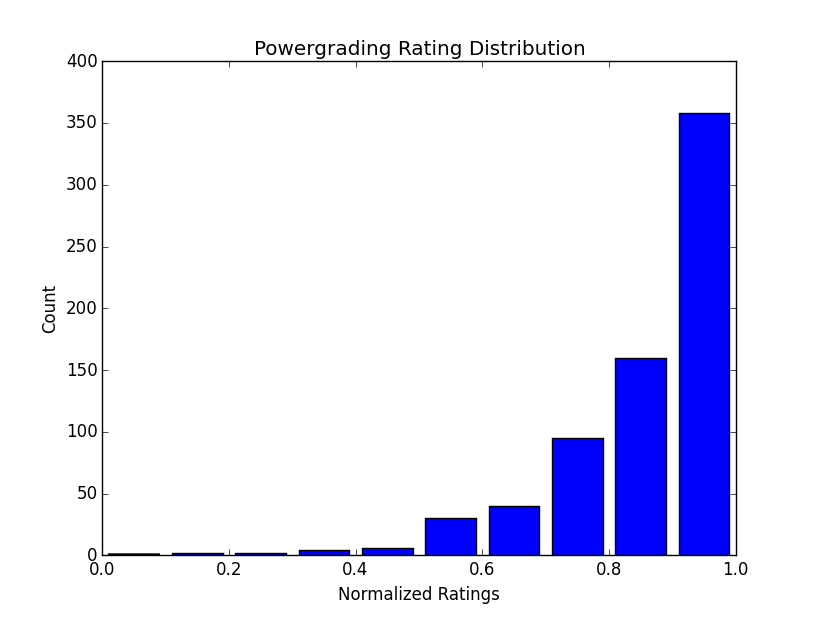
\includegraphics[width=0.5\textwidth]{figures/powerGradingDistribution.png}%
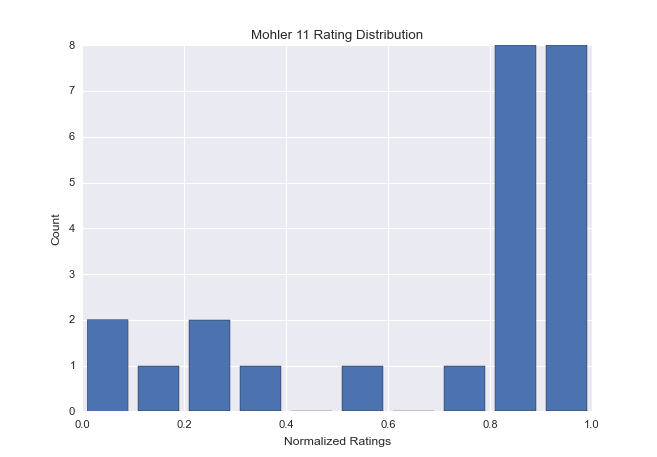
\includegraphics[width=0.5\textwidth] {figures/mohlerRatings.png}%
}%
\caption{Normalized ratings for two datasets used for evaluating approaches to the Luna Prediction Rating problem. The Powergrading dataset, comprised of responses to a subset of the 2012 United States Citizenship Exam, was introduced by Basu et al. (2013) \cite{basu2013powergrading}. The Mohler data, comprised of responses to problem set and exam questions in a University of North Texas Data Structures course, was introduced by Mohler et al. (2011) \cite{mohler2011learning}. Ratings were computed by summing individual question grades and normalizing.}
\label{fig:RatingDistribution}
\end{figure}

\subsection{Features}

Beyond stating LRP as a new problem for the machine learning community, the main contribution of this chapter is a thorough exploration of approaches to the problem. Following the recent work done on ASAG, my strategy is to associate several features with each set of responses, which can be subsequently used for regression. I divide the feature definitions into two categories: question-based features and response-based features. The former takes into account expected responses, while the latter focuses more on data provided by previous rated respondents. I then experiment with several types of regression to combine the features for an optimal model.

\subsubsection{Question-Based Features}
I assume now that Luna Game players have a set of expected answers for every question, which I refer to as an ``answer key''. The first time that the Luna Game is played with these questions, the player's only option is to compare the opponent's responses with the answer key. The closer a response is to the expected response, the higher the player's guess of their rating will likely be. Framed in this way, the problem becomes one of measuring the similarity between two samples of natural language.

Measuring semantic similarity between two samples of natural language can be a difficult task. If the two sentences differ only in word order, or only in a few words, then simple approaches can reliably detect similarity. By considering synonyms of the words in both sentences, the similarity measure may be improved. However, in many cases, it is impossible to accurately capture similarity without a deeper semantic understanding of the two sentences. One common approach for representing semantic similarities is to infer vector representations for words in the vocabulary of the training corpus, and then to calculate similarity based on some geometric measure, such as cosine similarity. The problem of inferring these vectors, referred to as neural embeddings, is an active area of research.

In the list below, I present all question-based features considered. In all cases, if there are multiple answers in the answer key, I take the maximum value over all possible values. All question-based features result in a vector whose length is equal to the number of questions in the dataset.

\begin{enumerate}
\item \textbf{Binary Word Overlap (BWO)}: The $i^{th}$ entry of this feature vector is 1 if any words in the $i^{th}$ response appear in the answer key and 0 otherwise.
\item \textbf{Fraction Word Overlap (FWO)}: The $i^{th}$ entry of this feature vector is the number of overlapping words in the $i^{th}$ response with the corresponding answer key, divided by the number of words in either the response or the answer key.  
\item \textbf{Character Edit Distance (CED)}: The $i^{th}$ entry of this feature vector corresponds to the edit distance (Levenshtein distance) between the $i^{th}$ response and the corresponding answer key at the level of characters. The value is 1.0 minus the fraction of the edit distance and the length of the larger string.
\item \textbf{Word Edit Distance (WED)}:  The $i^{th}$ entry of this feature vector corresponds to the edit distance (Levenshtein distance) between the $i^{th}$ response and the corresponding answer key at the level of words. For example, the WED between ``hello, world'' and ``goodbye, moon'' is 2. The value is 1.0 minus the fraction of the edit distance and the greater number of words in either string.
\item \textbf{Word2Vec Cosine Similarity (WCS)}: First I train a neural embedding of words using the answer key as a corpus. Then the $i^{th}$ response and the corresponding answer key are compared, and the $i^{th}$ entry of the feature vector is the maximum cosine similarity between the two. I use the library provided by Gensim here \cite{sojka2010software}.
\item \textbf{Semantic Nets (Li et al.) (SNL)}: For a more sophisticated approach to short sentence similarity, I refer to the work of Li et al. (2006) \cite{li2006sentence}. They offer a comprehensive metric that takes into account lexical, semantic, and syntactical information about the two sentences being compared. Their system is trained on a corpora of English sentences separate from the training data. I use an existing Python implementation of SNL that uses the bird2009natural English corpora \cite{bird2009natural}. The output of their similarity measure is a value between 0 and 1. Thus the $i^{th}$ entry of this feature vector contains the SNL similarity measure between the $i^{th}$ response and the corresponding answer key. One notable downside to this algorithm is that it takes significantly more time (up to 20x) than any other feature described in this chapter.
\end{enumerate}

One inherent challenge in the design of question-based features is the limited size of the answer key. At best, an answer key will document several responses that are considered completely correct. Unfortunately, for open-ended questions, the number of possible completely correct responses can be unbounded. Writing all possible correct responses becomes impractical and many responses may be incorrectly processed due to superficial differences with the answer key. Here I suggest two possible approaches to mitigating this problem. First, the answer key may be multiplied by applying various transformations, such as considering the synonyms of words in the original answer key or performing rearrangements in the syntax of the sentence. Second, as the training set increases, one may choose to include the answers of highly rated players in the answer key. In both cases, one should be sure that growing the answer key does not add prohibitive computational cost.

For future work on developing question-based features for LRP, it may be worthwhile to adapt methods for two related problems: paraphrase detection and textual entailment. Paraphrase detection assesses whether one sample is a paraphrase of the other. Textual entailment is the task of detecting whether one sample of natural language logically implies another sample. For our purposes, I might like to give high ratings to players whose responses imply the answer key, even if they are not exactly the same. Both of these problems are active areas of research in natural language processing and new results will likely be relevant to LRP as well.

\subsubsection{Response-Based Features}
As a player asks the same questions over several rounds, learning the opponent's true rating at the end of each round, the player's rating model should be updated to take into account the new data. For example, if a new set of responses is very similar to those of a previous opponent, the player's guess of the new opponent's rating should be close to the known rating of the previous opponent. Here I ignore the answer key and consider features that may be extracted solely from responses. In the list below, I present all response-based features tested. 

\begin{enumerate}

\item \textbf{Bag of Words (BOW)}: My simplest response-based feature is the standard natural language processing technique of Bag of Words. Given all the training data, I begin by creating a shared vocabulary list of all words that appear in any responses. I then associate a binary vector with each response in the training data, where entry $i$ is 1 if the response contains the $i^{th}$ word in the vocabulary and 0 otherwise.

\item \textbf{Bigrams (BIG)}: This feature is the same as BOW, except rather than building a vocabulary of single words, I build a vocabulary of two adjacent words.

\item \textbf{Bag of Synsets (SYN)}: This feature is similar to BOW. I create a thesaurus for every word in the generated vocabulary. I use the WordNet database for finding synonyms \cite{fellbaum1998wordnet}. Then I associate a vector for each response in the training data, where entry $i$ is 1 if the response contains any synonyms (including the word itself) of the $i^{th}$ word in the vocabulary.

\item \textbf{Nearest Neighbor via Overlap (NNO)}: This feature is based on the premise that similar responses will result in similar contributions to the respondents' ratings. For a given response, the most similar response in the training set is identified according to the number of overlapping words. The rating of the corresponding respondent is put into the feature vector, so that the final output is a vector containing the ratings of the most similar respondents per question.

\item \textbf{Nearest Neighbor via Character Edit Distance (NNC)}: This feature is the same as NNO, except similarity is defined by character edit distance rather than overlap.

\item \textbf{Nearest Neighbor via Word Edit Distance (NNW)}: This feature is the same as NNO, except similarity is defined by word edit distance rather than overlap.


\end{enumerate}

\subsection{Regression}
With features defined, the task then takes the standard form of a regression problem. For simplicity, I assume here that the rating is a linear combination of the features. I then consider two models of regression. The first is Ordinary Least Squares Linear Regression, which minimizes the sum of squares between predicted and actual ratings. I then run Lasso Regression $(\alpha = 0.1)$, which biases towards simpler models by penalizing the number of nonnegative coefficients in favor of sparse solutions. In both cases, I use the implementations in the Scikit-Learn library for machine learning \cite{pedregosa2011scikit}.
\section{Results}
I ran OLS Linear Regressions and Lasso Regressions on each of the 12 features for 100 trials. In addition, I included a combination of all 12 features (COM), and two controls. The first control predicts a random rating for a given set of responses (RAN). The second control, which I refer to as the ``constant best guess'', always predicts the average of all previously seen ratings (CBG). To consider a feature useful, it should at least outperform both of these controls on average. I define performance in terms of the Root Mean Square Error between predicted ratings and actual ratings in the test set. The results of these experiments are depicted in Figure 2. Lasso Regression yielded no meaningful differences from OLS, so I depict only the latter.
\begin{figure}[h]
\centerline{%
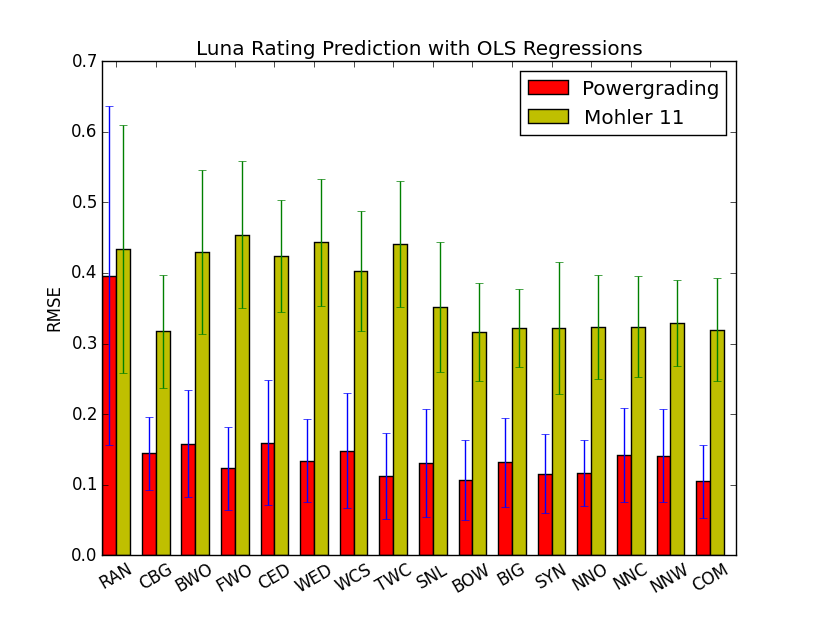
\includegraphics[width=0.9\textwidth]{figures/ratingPredictionFinalResults.png}%
}%
\caption{Fifteen approaches to the Luna Prediction Rating problem on two datasets using Ordinary Least Squares Linear Regression. From the left, the first two approaches represent baseline controls; the following six approaches are each OLS Linear Regressions on single question-based features; the following six are also OLS Linear Regressions, but on single response-based features instead; the last is an OLS Linear Regression that includes all 12 previous features. The Root Mean Square Error averaged over 100 trials is plotted for each approach. Refer to the text for the feature abbreviations.}
\label{fig:RatingDistribution}
\end{figure}

The relative performances of the approaches seem to be consistent between the two datasets tested. As expected, the Mohler 11 dataset proves far more difficult, likely due to the very limited size of the training set, the large number of responses per respondent, and the longer length of each response. Also unsurprising is the result that for OLS Linear Regression, a combination of all features outperforms any single feature. The combination does not perform as comparably well in Lasso Regression, presumably because the number of features actually included is small due to the penalty term. In both cases, any margin of improvement offered by a combination of all features is slim. Simple response-based features such as Bag of Words or Nearest Neighbor via Overlap are competitive with the combination. In practice, it may be preferable to use one or both of these due to the savings in computational resources. Among the question-based features, Binary Word Overlap fares the best, but cannot outperform the Constant Best Guess baseline. In future work, the question-based features could likely be improved by augmenting the answer keys as discussed above.

\section{Discussion}
In this chapter, I defined the Luna Rating Prediction problem of guessing a respondent's rating based on previous observations of responses and ratings. I discussed the closely related problem of Automatic Short Answer Grading and demonstrated how datasets and methods for ASAG can be adapted for LRP. I then presented initial work on LRP, which centered around several features of response sets that I use to learn a model for predicting ratings. These features were presented in two categories: question-based features, which rely only on a preset answer key, and response-based features, which ignore the answer key but take advantage of seen responses from previous rated respondents. I combined these features using traditional regression techniques to arrive at a comprehensive system for LRP.

For a player of the Luna Game, the ability to solve LRP is critical. The outcome of a Game hinges on the difference between predicted ratings and actual ratings. A human player may take advantage of the machine learning approaches to LRP offered here, but more likely the human will learn to rate well after several rounds of play without any formalisms or explicit machine learning. This human ability is based on an understanding of natural language, a deep knowledge base, and the relative ease with which humans judge one another in everyday scenarios. As machine players build an understanding of natural language and a knowledge base from answering questions in the Luna Game, these advances should be transferrable to LRP as well. A truly intelligent player of the Luna Game is unlikely to consider LRP and question answering as completely separate problems, but rather as manifestations of one general underlying problem.

Throughout this chapter, I sought to treat LRP as a general problem beyond the scope of the Luna Game, since I expect work on the problem to have several applications. Any situation in which a judge wishes to automatically evaluate a respondent can be thought of as an instance of LRP. The quantity being evaluated may be completely known to the respondent, as is the case in the Luna Game. However, in some applications, the quantity may be only partially known or unknown. For example, consider the case of a government official wishing to estimate the probability that a convict will repeat an offense based on questionnaire responses, or the case of an health insurance company wishing the estimate the amount of money that a customer will require for medical care. These real life applications combined with the motivation provided by the Luna Game make LRP a problem worthy of further study.
